\documentclass[fontsize=11pt,paper=a4,open=any,
twoside=no,toc=listof,toc=bibliography,headings=optiontohead,
captions=nooneline,captions=tableabove,english,DIV=12,numbers=noenddot,final,parskip=false,
headinclude=true,footinclude=false,BCOR=0mm]{scrartcl}
\pdfvariable suppressoptionalinfo 512\relax
\synctex=1

\author{Valentin Boettcher}
\usepackage{hirostyle}
\usepackage{hiromacros}
\addbibresource{references.bib}

\title{Input-Output Theory for Modulated Optical Fibre Resonators}
\date{2023}
\graphicspath{{graphics}}

\newcommand{\inputf}[0]{\ensuremath{\mathrm{in}}}
\newcommand{\outputf}[0]{\ensuremath{\mathrm{out}}}
\usetikzlibrary{math}
% \usetikzlibrary{external}
% \tikzexternalize[prefix=tikz/]
\usepackage{pgfplots}

\begin{document}
\maketitle
\tableofcontents

\section{Microscopic Derivation}
\label{sec:micr-deriv}
The setup we are describing consists of a general driven photonic
system \(A\) and a transmission line \(B\). The \(A\) system is
considered to have the Hamiltonian
\begin{equation}
  \label{eq:1}
  H_{A}=H_{0}+V(t) = ∑_{m} ω^{0}_{m} c_{m}^†c_{m} + V(t),
\end{equation}
where we are working in the basis that diagonalizes \(H_{0}\) and the
\(c_{m}\) are linear combinations of the bare modes in the photonic
system. We designate the bare modes of the EM field that are actually
in contact with the transmission line as \(a_{β}\) with
\begin{equation}
  \label{eq:4}
  E_{A}(x,t)= \iu \sqrt{\frac{\hbar}{2ε_{0}n_{A}^{2} L_{A,\perp}^{2} L_{A}}} ∑_{β}
  \sqrt{ω_{k_β}} \pqty{a_{β}(t)
    \eu^{\iu k_{β} x } - a_{β}^†(t)  \eu^{-\iu k_{β} x}},
\end{equation}
where \(L_{A,\perp}\) is a length scale that can be interpreted as the
diameter of the transmission line~\cite{Jacobs} and \(L_{A}\) is the
length of the cavity/resonator that hosts the electric field.  The
modes have wave numbers \(k_{β} = 2πβ/L_{A}\) for \(β \in \ZZ\) and
frequencies \(ω_{k_β} = c \abs{k_{β}}/n_{A}\), where \(n_{A}\) is the
refractive index inside the cavity. For simplicity we set \(\hbar
 = 1\) such that time is measured in units of inverse energy.

The bare \(a_{β}\) modes are linear combinations of the \(c_{m}\) and
can be related through
\begin{equation}
  \label{eq:5}
  a_{β} = ∑_{m} U_{βm} c_{m},
\end{equation}
where \(U\) is a not necessarily square matrix that obeys the
unitarity relation \(U U^† = \id\).  Transitioning into a rotating
frame with respect to \(H_{0}\) and employing the rotating wave
approximation removes all but the slowest-oscillating rotating terms
from the interaction
\begin{equation}
  \label{eq:12}
  \tilde{c}(t)_{m} = c_{m}(t)\eu^{\iu ω^{0}_{m}t}  \implies H_{A} \to \tilde{H}_{A}=
  ∑_{mn}V_{mn}(t) \eu^{-\iu t (ω^{0}_{n}-ω^{0}_{m})}
  \tilde{c}_{m}^†\tilde{c}_{n} \approx ∑_{mn}V^{0}_{mn} \eu^{\iu (ε_{m}-ε_{n})t}\tilde{c}_{m}^†\tilde{c}_{n}.
\end{equation}
Upon changing into another rotating frame we can remove this residual
time dependence
\begin{equation}
  \label{eq:33}
  h_{n}(t) = \tilde{c}_{n}\eu^{-\iu ε_{n}t} \implies \tilde{H}'_{A} =
  ∑_{mn}\bqty{V^{0}_{mn} + δ_{mn}ε_{m}} h_{m}^†h_{n}
\end{equation}

We can subsequently find a unitary transformation that diagonalizes
the RWA interaction
\begin{equation}
  \label{eq:30}
  ∑_{mn}\pqty{O^{†}}_{im}\bqty{V^{0}_{mn} + δ_{mn}ε_{m}}O_{nj} = ω_{j} δ_{ij},
\end{equation}
where the columns of \(O\) are the normalized eigenvectors of
\(V_{mn}^{0}=\mel{m}{V^{0}}{n}\). So if \(\ket{ψ_{j}}\) is an
eigenvector of \(V\), then \(\braket{i}{ψ_{j}} = O_{ij}\)
\footnote{This is just a reminder for Valentin who can't seem to keep
  this in his head.}.

Transforming the \(h_{m}\) according to
\begin{equation}
  \label{eq:13}
  d_{γ} = ∑_{n}O^{\ast}_{nγ}(0) h_{n} = ∑_{n}O^{\ast}_{nγ}(t) \tilde{c}_{n}  \implies \tilde{H}''_{A} = ∑_{γ}ω_{γ} d_{γ}^†d_{γ}
\end{equation}
where
\begin{equation}
  \label{eq:35}
  O^\ast_{nγ}(t)\equiv O^\ast_{nγ}\eu^{-\iu ε_{n}t}
\end{equation}
leaves us with a very simple Hamiltonian.

Let us list the relation between the \(a\), \(c\), \(h\) and \(d\) operators
for later reference
\begin{align}
  \label{eq:15}
  c_{n} &= \eu^{-\iu
          ω^{0}_{n} t}\tilde{{c}}_{n} = \eu^{-\iu
          (ω^{0}_{n}-ε_{n}) t} h_{n}=  \eu^{-\iu
          (ω^{0}_{n}) t} ∑_{γ} O_{nγ}(t)d_{γ} \\
  a_{β} &= ∑_{m} U_{β,m} c_{m} = ∑_{m} U_{β,m} \tilde{c}_{m}\eu^{-\iu
          ω^{0}_{m} t} = ∑_{mγ} U_{β,m} \eu^{-\iu
          ω^{0}_{m} t} O_{mγ}(t)d_{γ}
\end{align}


The transmission line is considered to only
have one polarization direction and one dimension of
propagation, so that the vector potential is effectively scalar and we
have
\begin{equation}
  \label{eq:2}
  E_{B}(x, t) = \iu\sqrt{\frac{\hbar}{2ε_{0}n_{B}^{2}
      (2π)^{3}L_{B,\perp}^{2}}}  ∫{\sqrt{ω^{B}_{k}}} \pqty{b_{k}(t)
    \eu^{\iu k x } - b_{k}^†(t)  \eu^{-\iu k x}}\dd{k},
\end{equation}
with \(\comm{b_{k}}{b_{q}^†}=δ(k-q)\), \(ω^{B}_{k} = c \abs{k}/n_{B}\)
with \(n_{B}\) being the refractive index of the fibre and
\(L_{B,\perp}\) being the perpendicular length scale as discussed
above. Note that the \(b_{k}\) here have dimensions of \(\sqrt{[L]}\)
as opposed to \(\sqrt{[t]}\), as is the usual convention in
input-output theory. If a stochastic theory is desired, the latter
convention is preferrable and can be obtained through substituting
\(k\to \pm ω/c n_{B}\) and rescaling
\(b_{k}\to b_{k}/ \sqrt{c n_{B}^{-1}}\).

An interaction between the transmission line and the
system \(A\) roughly inspired by coupled mode theory is
\begin{equation}
  \label{eq:3}
  H_{I} = g_{0} ∫ E_{A,+}(x,t)E_{B,-}(x,t) f(x) \dd{x} + \hc,
\end{equation}
where the subscripts \(\pm\) denote positive or negative frequency
portions of the fields and \(f(x)\) is a dimensionless weighting
function with compact support \([-Δx/2, Δx/2]\) whose maximum is
unity.  Coupling only the positive/negative parts simplifies the
calculations and is consistent with the later application of the
rotating wave approximation. A possible phase shift between the fields
has been absorbed into the definition of the creation and annihilation
operators.

Expanding the fields in \cref{eq:3} we obtain
\begin{equation}
  \label{eq:6}
  H_{I} = {g_{0}} \frac{\hbar Δx}{2 ε_{0}n_{A}n_{B} (2π)^{3}
    L_{A,\perp}L_{B,\perp}\sqrt{L_{A}}}  ∑_{β}∫
  \sqrt{ω^{B}_{k}ω_{k_{β}}}\,\tilde{f}(k-k_{β})\,  b^†_{k}
  a_{β} \dd{k} + \hc
\end{equation}
The Fourier transform of the weighting function
\begin{equation}
  \label{eq:7}
  \tilde{f}(k) = \frac{1}{Δx} ∫f(x)\eu^{-\iu k x} \dd{x}
\end{equation}
controls how ``far'' the interaction reaches in \(k\)-space. In the
extreme case \(Δx\to 0\) every \(b_{k}\) couples to every \(a_{β}\),
whereas for \(Δx\to ∞\) only modes with matching wave-numbers
couple. As the \(b_{k}\) will contain both the coherent drive with a
laser and the output field amplitudes it is desirable to have this
coupling to be as local in \(k\)-space as possible for targeted
control and precise readout. In the limit of weak coupling between
transmission line and system, which we will assume in a short while,
the rotating wave approximation will ensure that our result won't
depend significantly on the choice of \(f\).

The coupling constant \(g_{0}\) in \cref{eq:6} has the dimensions of
\([L]^{2}\times [ε_{0}]\). We define a new coupling constant that has
units of energy as
\begin{equation}
  \label{eq:8}
  g_{0} = g\frac{n_{A}n_{B}ε_{0} L_{A,\perp}L_{B,\perp} 2(2π)^{3}}{\hbar ω_{0}},
\end{equation}
where \(ω_{0}\) is a typical frequency\footnote{For example, the
  frequency of the drive laser.}.
Using this, \cref{eq:6} becomes
\begin{equation}
  \label{eq:9}
  \begin{aligned}
    H_{I} &= \frac{gΔx}{
     \sqrt{L_{A}}}  ∑_{β}∫
    G_{β}(k)  b^†_{k}
    a_{β} \dd{k} + \hc
    &G_{β}(k) &= \frac{\sqrt{ω^{B}_{k}ω_{k_β}}}{ω_{0}} \tilde{f}(k-k_{β}).
  \end{aligned}
\end{equation}
We note that for
a \(ω_{k_{β}}= ω_{0} + δω\) with \(δω \ll ω_{0}\) the coupling factor
\(G_{β}(k)\) only depends on the difference \(k-k_{β}\). By defining
\begin{equation}
  \label{eq:11}
  \mathcal{O(k)} = \frac{Δx}{\sqrt{L_{A}}} ∑_{β} G_β(k)a_{β} =
  \frac{Δx}{\sqrt{L_{A}}} ∑_{β,m} G_β(k)U_{β,m}c_{m}
\end{equation}
the interaction takes on the more familiar form
\begin{equation}
  \label{eq:14}
  H_{I} = {g}  ∫
   b^†_{k} \mathcal{O}(k)
  \dd{k} + \hc
\end{equation}

Changing variables from \(k\) to\footnote{This is a bit
  unconventional.} \(ω^{B}_{k}=k c / n_{B}\) in
\cref{eq:9} we obtain
\begin{equation}
  \label{eq:17}
  H_{I} = \frac{gΔx}{\sqrt{L_{A}}}  ∑_{β}∫_{-∞}^{∞}
   G'_{β}(ω)f^†_{ω}
  {a_{β}} \dd{ω} + \hc,
\end{equation}
where \(f_{ω}=\sqrt{\frac{n_{B}}{c}}b_{\frac{ω n_{B}}{c}}\) with
\(\comm{f_{ω}}{f_{ω'}^†}=δ(ω-ω')\) and
\(G'_{β}(ω)=G_{β}\pqty{\frac{ω n_{B}}{c}}\).


\subsection{Rotating Wave and First Markov Approximation}
\label{sec:rotating-wave-first}
Following the route taken in \cite{Jacobs}, the next step would be to
transition into a rotating frame so that
\(\tilde{H}_{A}=\tilde{H}_{B}=0\) and apply the rotating wave
approximation. Here, the rotating terms that would occur have the
frequencies of the form \(ω^{0}_m + ω_{γ}\) which are not guaranteed
to be spaced sufficiently far apart for the RWA to
apply\footnote{Consider, for example the SSH model where the
  \(k\)-space density can be arbitrarily high depending on the length
  of the chain.}. We therefore work in the frame of the
\(\tilde{c}_{m}\) and \(\tilde{f}_{ω} = f_{ω}\eu^{\iu \abs{ω}t}\) to
obtain
\begin{equation}
  \label{eq:10}
  \tilde{H}_{I}= \frac{gΔx}{
    \sqrt{L_{A}}}  ∑_{β,m}∫
  G'_{β}(ω)  \eu^{-\iu
    (ω^{0}_{m}-\abs{ω}) t}
  U_{β,m} \tilde{f}_k^†\tilde{c}_{m} \dd{ω} + \hc
\end{equation}

\begin{figure}[H]
  \centering
  {\fontsize{8pt}{1em}
  \input{graphics/rwa_illustr.pdf_tex}}
\caption{\label{fig:rwa_illustr} In the rotating wave approximation
  The bare frequencies of the resonator only couple to the
  transmission line in frequency sub-intervals
  \([ω_{m}-λ_{m}, ω_{m}+λ_{m}]\).  A second effect that comes into
  play is the geometrically induced coupling amplitude \(\tilde{G'}_{m}(ω)\),
  which is visualized around \(ω_{m}\) under the assumption \(ω_{β}
  \approx ω_{0}^{m}\) for some small range of \(m\).}
\end{figure}
For \(g \ll ω_{m}^{0}\) each \(\tilde{c}_{m}\) in \cref{eq:10} only
interacts with non-overlapping sub-intervals
\([ω^{0}_{m}-λ_{m}, ω^{0}_{m}+λ_{m}]\) of the transmission frequency axis
(rotating wave approximation) with \(g\ll λ_{m} \ll ω_{m}^{0}\). This
situation is illustrated in \cref{fig:rwa_illustr}. Also, the coupling
amplitude \(G_{β}(ω)\) is local in frequency space and can assist the
RWA depending on the choice of parameters and how close the
\(ω^{0}_{m}\) are to the \(ω_{k_{β}}\). We obtain
\begin{equation}
  \label{eq:16}
  \tilde{H}_{I}\approx \frac{gΔx}{
    \sqrt{L_{A}}}  ∑_{β,m}∫_{ω^{0}_{m}-λ_{m}}^{ω^{0}_{m}+λ_{m}}
  \eu^{-\iu
    (ω^{0}_{m}-\abs{ω}) t}
  U_{β,m} \pqty{G'_{β}(ω)  \tilde{f}_{ω}^† + G'_{β}(-ω)
    \tilde{f}_{-ω}^†}\tilde{c}_{m} \dd{ω} + \hc
\end{equation}
For any finite \(Δx\) and
\(ω_{0}^{m},ω_{k_{β}}\gg \frac{2πc}{Δx n_{A}}\) we can assume
\begin{equation}
  \label{eq:44}
  G'_{β}\pqty{-\sgn(β)  ω}\approx 0
\end{equation}
in \cref{eq:16}.

As each \(\tilde{c}_{m}\) is now interacting with non-overlapping
transmission-line field modes, we can introduce a separate field for
each \(\tilde{c}_{m}\) that commutes with all other fields and extend
the integration bounds to infinity again\footnote{This is called the
  ``First Markov Approximation'' in \refcite{Gardiner1985}.}.
Care has to be taken to maintain consistency with \cref{eq:44},
\begin{equation}
  \label{eq:16}
  \tilde{H}_{I}= \frac{gΔx}{
    \sqrt{L_{A}}}  ∑_{β,m}∫_{0}^{∞}
  \eu^{-\iu
    (ω^{0}_{m}-\abs{ω}) t}
  U_{β,m} G'_{β}(\sgn({β})ω)  \tilde{f}^{m,†}_{\sgn({β})ω}{c}_{m} \dd{ω} + \hc
\end{equation}
which becomes\footnote{A lot of discussion for a simple result :).}
\begin{equation}
  \label{eq:18}
  H_{I}= ∑_{m}∫_{-∞}^{∞}
  \tilde{G}_{m}(k) {b}^{m,†}_{k}{c}_{m} \dd{k}
\end{equation}
upon transitioning out of the rotating frame with \(\tilde{G}_{m}(k) =
\frac{gΔx}{
  \sqrt{L_{A}}}  ∑_{β\gtrless 0}U_{β,m} G_{β}(k)δ_{\sgn(β),\sgn(k)}\). The equation of motion
for the transmission line modes become
\begin{gather}
  \iu\dot{b}^{m}_{k} = ω^{B}_{k} b_{k}^{m,†} +
  \tilde{G}_{m}(k) c_{m}\\
    \label{eq:19}
  \implies b^{m}_{k}(t) = b^{m}_{k}(0) \eu^{-\iu ω_{k}^{B}t} -\iu
  \tilde{G}_{m}(k) ∫_{0}^{t}\eu^{-\iu
    ω_{k}^{B}(t-s)} c_{m}(s)\dd{s}.
\end{gather}
The equation of motion for \(\tilde{c}_{m}\) is
\begin{equation}
  \label{eq:21}
  \iu\dot{\tilde{c}}_{m} = ∑_{n}V^{0}_{mn} \tilde{c}_n +
  \underbrace{\eu^{\iu ω_{m}^{0}t}∫_{-∞}^{∞}\tilde{G}^\ast_{m}(k)
    b_{k}^{m}(t)\dd{k}}_{\equiv I}.
\end{equation}
Further inspection of the rightmost term in \cref{eq:21} yields
\begin{equation}
  \label{eq:22}
  \begin{aligned}
    I &= \eu^{\iu ω_{m}^{0}t} ∫_{-∞}^{∞}\tilde{G}^\ast_{m}(k)
        b_{k}^{m}(t)\dd{k} \\
      &= ∫_{-∞}^{∞}\tilde{G}^\ast_{m}(k)
        b_{k}^{m}(0)\eu^{-\iu (ω^{B}_{k} - ω^{0}_{m})t}\dd{k} -\iu  ∫_{0}^{t}∫_{-∞}^{∞}\abs{\tilde{G}_{m}(k)}^{2}
        \tilde{c}_{m}(s)\eu^{-\iu ω^{B}_{k}(t-s)} \eu^{\iu
        ω^{0}_{m}(t-s)}\dd{k}\dd{s}\\
       &=II + III.
  \end{aligned}
\end{equation}
Inspired by the RWA, we now assume
\begin{equation}
  \label{eq:23}
  \begin{aligned}
    \tilde{G}_{m}(k) &\approx
    δ_{m}\tilde{G}_{m}\pqty{\sgn(k) ω_{m}^{0}\frac{n_{B}}{c n_{A}}} =
    δ_{m}\frac{gΔx}{\sqrt{L_{A}}}∑_{β}U_{βm}G_{β}\pqty{\sgn(k) ω_{m}^{0}\frac{n_{B}}{c
    n_{A}}} δ_{\sgn(β),\sgn(k)} \\
    &\equiv ∑_{β}g^{0}_{β} U_{βm}δ_{\sgn(β),\sgn(k)} \equiv g_{m, \sgn(k)}
  \end{aligned}
\end{equation}
in the interval \([ω^{0}_{m}-λ_{m}, ω^{0}_{m}+λ_{m}]\) (see
\cref{eq:16}) where \(δ_{m}\) is a possible scaling factor to better approximate
\(\tilde{G}_{m}(k)\) as a constant in \cref{eq:16}.

Additionally we resurrect\footnote{Within
  the RWA this is all equivalent, but I prefer having the input field
  proportional to the electric field!} the \(ω_{k}^{B}\) dependence of
\(G_{m}(k)\) in \(I\) to obtain
\begin{equation}
  \label{eq:24}
  \begin{aligned}
    II &= \frac{\eu^{\iu ω_{m}^{0}t}}{\sqrt{ω_{m}^{0}}} \bqty{g_{m,+}^\ast ∫_{0}^{∞}\sqrt{ω^{B}_{k}}b^{m}_{k}(0)\eu^{-\iu
    ω^{B}_{k}t}\dd{k} + g_{m,-}^\ast∫_{-∞}^{0}\sqrt{ω^{B}_{k}}b^{m}_{k}(0)\eu^{-\iu
         ω^{B}_{k}t}\dd{k}}\\
    &\equiv \frac{\eu^{\iu ω_{m}^{0}t}}{\sqrt{ω_{m}^{0}}}\pqty{
      g_{m,+}^\ast b_{\inputf,+}^{m}(t) + g_{m,-}^\ast b_{\inputf,-}^{m}(t)},
  \end{aligned}
\end{equation}
where \(b_{\inputf,+(-)}^{m}(t)\) is identified as the
right(left)-moving input field and is proportional to the annihilation
part of the electric field. The second part of \cref{eq:22} becomes
\begin{equation}
  \label{eq:25}
  III= -\iu ∫_{0}^{t}\eu^{\iu ω^{0}_{m}(t-s)}\tilde{c}_{m}(s)
  \bqty{ \abs{g_{m,+}}^{2} ∫_{0}^{∞}\eu^{-\iu ω^{B}_{k}(t-s)} \dd{k} + \abs{g_{m,-}}^{2}  ∫_{-∞}^{0}\eu^{-\iu ω^{B}_{k}(t-s)} \dd{k}}\dd{s}.
\end{equation}
Now we use the identity
\begin{equation}
  \label{eq:26}
  ∫_{0}^{∞}\eu^{-\iu ω^{B}_{k}(t-s)} \dd{k} = \frac{n_{B}}{c}
  \bqty{\mathcal{P}\frac{-i}{t-s} + π δ(t-s)},
\end{equation}
but neglect the principal value, as it leads only to rapidly
oscillating terms that are inconsistent with the RWA, to obtain
\begin{equation}
  \label{eq:27}
  III= -2\iu η_{m}∫_{0}^{t}\eu^{\iu ω^{0}_m(t-s)}\tilde{c}_{m}(s)
  δ(t-s)\dd{s} = -\iu η_{m} \tilde{c}_{m}(t),
\end{equation}
where the factor \(1/2\) in the last equality stems from the fact that
we only use half of the delta function and
\begin{equation}
  \label{eq:45}
  η_{m}\equiv π\frac{n_{B}}{c}\bqty{\abs{g_{m,-}}^{2}+\abs{g_{m,+}}^{2}}.
\end{equation}
Note that \cref{eq:45} is an incoherent sum of the couplings to the
right moving and left moving fields in the transmission line.
Altogether we arrive at
\begin{equation}
  \label{eq:28}
  \dot{\tilde{c}}_{m} = -\iu\bqty{∑_{n}V^{0}_{mn} \tilde{c}_n +
    \frac{\eu^{\iu ω_{m}^{0}t}}{\sqrt{ω_{m}^{0}}}
    ∑_{σ=\pm}g_{m,σ}^\ast b_{\inputf,σ}^{m}(t)} - η_{m}\tilde{c}_{m}.
\end{equation}
The usual situation is that \(b^{m}_{\inputf, -} = 0\) and we can
restrict ourselves to the coupling to the right-moving input field.

\subsection{Input-Output Relation and further Simplifications}
\label{sec:input-outp-relat}
Integrating \cref{eq:19} over all \(k\) yields
\begin{equation}
  \label{eq:29}
  \begin{aligned}
    \frac{b_{\outputf}^{m}(x,t)}{\sqrt{ω^{0}_{m}}} &\equiv
  \frac{1}{\sqrt{ω_{m}^{0}}}∫ \sqrt{ω^{B}_{k}} b_{k}^{m}(t) \eu^{\iu k
                                                     t}\dd{k}\\
    &=
  \frac{1}{\sqrt{ω_{m}^{0}}} b_{\inputf}^{m}(x, t) -\iu
      g_{m,\sgn(x)}\frac{π n_{B}}{c}
      \tilde{c}_{m}(τ(x,t))\eu^{-i ω^{0}_{m}τ(x,t)}Θ(τ(x,t)),
  \end{aligned}
\end{equation}
which is the input-output relation with the retarded time
\begin{equation}
  \label{eq:20}
  τ(x,t)=t - \frac{\abs{x}n_{B}}{c}.
\end{equation}
The coupling constant accounts for the direction of propagation and
the time argument is properly retarded. We defined
\begin{equation}
  \label{eq:48}
  b_{\inputf}^{m}(x,t) = ∫\sqrt{ω^{B}_{k}} b_{k}^{m}(0)\eu^{\iu \pqty{kx -
    ω_{k}^{B}t}}\dd{k}
\end{equation}
used that
\begin{equation}
  \label{eq:42}
  ∫_{0}^{∞}\eu^{-\iu ω^{B}_{k}(t-s)}\eu^{\pm\iu k x} \dd{k} =
  \frac{n_{B}}{c}
  \bqty{\mathcal{P}\frac{-i}{t-s \pm \frac{x n_{B}}{c}} + π δ\pqty{t-s\mp
    \frac{x n_{B}}{c}}}.
\end{equation}

The case of \(x=0\) is recovered by defining
\begin{equation}
  \label{eq:47}
  \lim_{x\to0} g_{m,\sgn(x)=0} = \frac{1}{2} \pqty{g_{m,+} + g_{m,-}},
\end{equation}
which amounts to taking half of each delta function in
\cref{eq:42}. It shall be noted, that it is physical to assume
\(x>0\), as we necessarily measure outside the fibre-coupler between
transmission line and resonator. By neglecting the \(k\)-depnedence of
the coupling in \cref{eq:23} through invocation of the RWA we have
effectively ignored length \(Δx\), but to maintain consistency with
\cref{eq:44} we should assume it to be finite.
We can also neglect the retardation if \(x / v_{g}\) is
much smaller than a typical timescale we're interested in.


To integrate \cref{eq:28}, we
first diagonalize \(V^{0}_{mn} + δ_{mn}\pqty{ε_{m}-i η_{m}}\)
\begin{equation}
  \label{eq:65}
  V^{0}_{mn} + δ_{mn}\pqty{ε_{m}-i η_{m}} \to ∑_{γγ'}
  δ_{γγ'}(ω_{γ}-\iu \tilde{n}_{γ})
\end{equation}
to obtain \(O_{mγ}(t)\) and find
\begin{equation}
  \label{eq:32}
  \dot{d}_{γ} = ∑_{m}\pqty{O^{-1}(t)}_{γm}\dot{\tilde{c}}_{m} =
  -\iu\bqty{\pqty{ω_{γ} - \iu \tilde{η}_{γ}}d_{γ} +
    ∑_{σ=\pm}∑_{m}\pqty{O^{-1}(t)}_{γm}\frac{g_{m,σ}^\ast }{\sqrt{ω_{m}^{0}}} \eu^{\iu ω_{m}^{0}t}
    b_{\inputf,σ}^{m}(t)}.
\end{equation}

We now introduce some additional simplifications beginning with
equating all input fields \(b_{\inputf}^{m}\). This is allowed, as we
will transition to the classical picture later, where the commutation
relations do not matter. We also assume that we're working in a region
in \(m\) space, where the \(g_{β}^{0}\approx \sqrt{κ}\) and
\(\sqrt{ω^{0}_{m}}\approx\sqrt{ω_{0}}\), where \(ω_{0}\) is a typical
frequency in the input field, can be assumed to be approximately
constant. With these considerations in mind we can simplify
\cref{eq:32} to
\begin{equation}
  \label{eq:64}
  η_{m}=\abs{κ}\frac{πn_{B}}{c}∑_{σ=\pm,β,β'}U_{βm}U^\ast_{β'm}δ_{\sgn(β),σ} δ_{\sgn(β'),σ}
\end{equation}
and
\begin{gather}
  \label{eq:34}
  \dot{d}_{γ} =
  -\iu\bqty{\pqty{ω_{γ}-\iu \tilde{η}_{γ}}d_{γ} + \sqrt{κ^\ast} ∑_{σ=\pm}
    U^{σ}_{γ}(t) \frac{b_{\inputf}(t)}{\sqrt{ω_{0}}}}\\
  U^{σ}_{γ}(t) = ∑_{m,β} δ_{\sgn({β}),σ}U^\ast_{βm}\pqty{O^{-1}(t)}_{γm} \eu^{\iu ω_{m}^{0}t}= ∑_{m,β} δ_{\sgn({β}),σ}U^\ast_{βm}\pqty{O^{-1}}_{γm}\eu^{\iu (ω_{m}^{0}-ε_{m})t}.
\end{gather}

These simplifications still capture the essence of the physics, as
demonstrated in the current long-range SSH experiment.

We can now proceed to integrate \cref{eq:34} to obtain
\begin{equation}
  \label{eq:36}
  d_{γ}(t)= d_{γ}(0) \eu^{-\pqty{\iu ω_{γ} + \tilde{η}_{γ}}t} -
  \frac{i}{\sqrt{κ}} Σ_{σ=\pm} ∫_{0}^{t}χ_{γ}(t-s) U^{σ}_{γ}(s)
  \frac{b_{\inputf,σ}(t)}{\sqrt{ω_{0}}}\dd{s}
\end{equation}
with
\begin{equation}
  \label{eq:37}
  χ_{γ}(t) = \abs{κ} \eu^{-\pqty{\iu ω_{γ} + \tilde{η}_{γ}}t}.
\end{equation}

When constructing the total output field, we have to remember how the
separate fields \(b_{\outputf,m}\) came about. We assumed that each
\(c_{m}\) only interacted with a finite range of modes (see
\cref{eq:16}) in the transmission line and then just extended the
resulting sub-fields back to full independent fields for
simplicity. Now, we have to perform the reverse process, which amounts
to summing together all system (resonator) contributions in
\cref{eq:34} as these only excite the sub-fields and we can safely
glue them back together. To be consistent, we have to sum together the
finite ranges of the input fields which amounts to having \emph{one}
whole copy of the input field.
This leads us to
\begin{equation}
  \label{eq:38}
  \frac{b_{\outputf}(x,t)}{\sqrt{ω_{0}}} \equiv
  \frac{1}{\sqrt{ω_{0}}} b_{\inputf}(x, t) -i  θ(τ(x,t)) \frac{\sqrt{κ}πn_{B}}{c}
  ∑_{γ}\bqty{U^{\sgn(x)}_{γ}\pqty{τ(x,t)}}^\ast d_{γ}(τ(x,t))
\end{equation}

Transitioning to expectation values and using \(\ev{d_{γ}(0)}=0\) we
find
\begin{equation}
  \label{eq:39}
  \ev{{b_{\outputf}(x,t)}} =
  \ev{b_{\inputf}(x,t)} - ∑_{σ=\pm}∫_{0}^{τ(x,t)}χ_{\sgn(x),σ}(τ(x,t),s) \ev{b_{\inputf,σ}(s)} \dd{s}
\end{equation}
with the time non-local susceptibility for the left and right moving
input fields
\begin{equation}
  \label{eq:40}
  χ_{δ,σ}(t,s) = \frac{π n_{B}}{c}Θ(t) ∑_{γ}\pqty{U^{δ}_{γ}(t)}^\astχ_{γ}(t-s)U^{σ}_{γ}(s).
\end{equation}

For an input field with no left-moving components and a measurement
position \(x>0\) we have
\begin{equation}
  \label{eq:31}
  \ev{{b_{\outputf}(x>0,t)}} =
  \ev{b_{\inputf}(x,t)} -∫_{0}^{τ(x,t)}χ_{++}(τ(x,t),s) \ev{b_{\inputf}(s)} \dd{s}.
\end{equation}
with \(b_{\inputf}(s) = b_{\inputf,+}(s) + b_{\inputf,-}(s) = b_{\inputf,+}(s)\).

\section{Application to the Non-Markovian Quantum Walk}
\label{sec:appl-non-mark}
The experimental setup for implementing the non-Markovian quantum walk
discussed in~\cite{Ricottone2020,Kitagawa2010} is illustrated in
\cref{fig:schematic}. The abstract system introduced in
\cref{sec:micr-deriv} is replaced by a small \(S\) and a large \(B\)
fibre loop with lengths \(L_{B}\gg L_{S}\). The resonant modes of the
loops do have the free spectral ranges
\begin{equation}
  \label{eq:41}
  \begin{aligned}
    Ω_{B} &= \frac{2πc}{n_{B}} & Ω_{S} &= \frac{2πc}{L_{S}},
  \end{aligned}
\end{equation}
where \(n\) is the refractive index of the respective fibres.
\begin{figure}[htp]
  \centering
  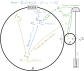
\includegraphics{walker_setup}
  \caption{\label{fig:schematic}Schematic of the experimental setup.}
\end{figure}
Attaching the transmission line to the smaller loop has the advantage
that we only excite and detect what we will later identify as the
\(A\) level of the non-Markovian quantum walk in momentum space.

We assume that the loops share some common eigenfrequency
\begin{equation}
  \label{eq:46}
  ω_{s} = n_{0}^{S}Ω_{S} = n_{0}^{B}Ω_{B}\iff \frac{n_{0}^{B}}{L_{B}}
  = \frac{n_{0}^{S}}{L_{S}}
\end{equation}
with \(n,m\gg 1\) and \(ω_{s}\) close to the frequency of the
laser. We choose to index the eigenfrequencies of the loops relative
to \(ω_{s}\) so that
\begin{equation}
  \label{eq:49}
  \begin{aligned}
    ω_{n}^{X} &= ω_{s} + n Ω_{X} & k_{n}^{X} = \frac{2π}{L_{B}}
                                   n_{0}^{X} + \frac{2π}{L_{B}} n = k_{0} + \frac{2π}{L_{B}} n,
  \end{aligned}
\end{equation}
where \(X=S,B\).

These loops are coupled to each other with amplitude \(δ\eu^{\iu ϕ}\) which can
possibly contain a phase due to the choice of the coordinate
origin. Let us now assume that
\begin{equation}
  \label{eq:50}
  \frac{Ω_{S}}{Ω_{B}} = 2N+1
\end{equation}
with \(N\in \NN\). We denote by \(a\) the annihilation operator for the
mode with \(ω=ω_{s}\) in the small loop and suppress all other modes
in the small loop, as we will not populate them. The annihilation
operators \(f_{n}\) destroy modes with frequencies \(ω^{B}_{n}\) in
the big loop, where we limit \(n\) to the range \([-N, N]\) for the
same reasons as above.
This leads to the Hamiltonian
\begin{equation}
  \label{eq:51}
  H_{A}= ω_{s}a^†a + ∑_{n=-N}^{N} ω_{n}^{B}f_{n}^†f_{n} + δ \pqty{\eu^{\iu
    ϕ}f_{0}^†a + \eu^{-\iu ϕ}a^†f_{0}} + ∑_{mn}J_{mn}(t) f_{m}^†f_{n},
\end{equation}
where \(J_{mn}(t)\) is the coupling mediated by the EOM in the big
loop. The phase \(ϕ=k_{0}L_{S}/2\) of the coupling stems from the
location of the fibre coupler along the loop but can potentially also
contain other contributions.

To be bring the Hamiltonian into the form \cref{eq:1}, we define
\begin{equation}
  \label{eq:52}
  \begin{aligned}
    c_{\pm} &= \frac{1}{\sqrt{2}}\pqty{f_{0}\eu^{-\iu ϕ} \pm a} &
                                                                  c_{n\neq
                                                                  0}&=f_{n}\\
    ω_{\pm}^{0}&=ω_{s}\pm δ & ω_{n\neq 0}&= ω_{s} + Ω_{B} n\\
    V_{\pm,\pm}&=\frac{J_{00}}{2} & V_{\pm, n\neq0} &=
                                                      \frac{J_{0n}}{\sqrt{2}}\eu^{\iu
                                                      ϕ}\\
    V_{n\neq \pm, m\neq \pm} &= J_{nm}
  \end{aligned}
\end{equation}
and obtain
\begin{equation}
  \label{eq:54}
  H_{A} = ∑_{n} ω_{n}^{0}c_{n}^†c_{n} + ∑_{nm} V_{nm}(t) c_{n}^†c_{m},
\end{equation}
where the index \(n\) can take on the values in
\(\pqty{[-N,N]\setminus \{0\}} \cap \{+, -\}\). The spectra of the
coupled and uncoupled systems are visualized in \cref{fig:spectra}.

\tikzmath{
  \Nmodes = 5;
  integer \NmodesBetween;
  \NmodesBetween = \Nmodes - 1;
  \delta = .2;
}
\begin{figure}[p]
  \centering
\begin{tikzpicture}[y=-1.5cm]
  \draw[->] (-1.5, -1) -- node[left] {\(ω\)} ++(0,2);

  \foreach \y in {-\Nmodes,...,\Nmodes}
  \draw  (0, \y) node[left] {\(ω^{B}_{\y}\)} -- ++(1, 0);

  \foreach \y/\name in {-\Nmodes/-1,0,\Nmodes/1}
  \draw (1.1, \y) -- ++(1, 0) node[right] {\(ω^{S}_{\name}\)};
\end{tikzpicture}
\begin{tikzpicture}[y=-1.5cm]
  \foreach \y in {-\NmodesBetween,...,-1}
  \draw  (0, \y) node[left] {\(ω^{0}_{\y}\)} -- ++(1, 0);

  \foreach \y in {1,...,\NmodesBetween}
  \draw  (0, \y) node[left] {\(ω^{0}_{\y}\)} -- ++(.5, 0) node(mc\y){}
  -- ++(.5, 0) node(mr\y){};

  \foreach \y in {-\Nmodes,\Nmodes} {
    \foreach \sub/\name in {-\delta/-, \delta/+}
    \draw  (0, \sub+\y) --  ++(.5, 0)  -- ++(.5, 0);
  }

  \foreach \y in {0} {
    \foreach \sub/\name in {-\delta/-, \delta/+}
    \draw (0, \sub+\y) node[left] {\(ω^{0}_{\name}\)} --  ++(.5, 0) node(pmc\name){} -- ++(.5, 0) node[right] (pmr\name){};
  }

  \foreach \y in {-\Nmodes,0,\Nmodes}
  \draw[dashed,color=gray]  (0, \y) -- ++(1, 0);

  \draw[<->] (pmc+) -- node[right] {\(2δ\)} (pmc-);
  \draw[<->] (pmc+) -- node[right] {\(Ω_{B} - δ\)} (mc1);
  \draw[<->] (mc1) -- node[right] {\(Ω_{B}\)} (mc2);
\end{tikzpicture}
\caption{\label{fig:spectra}The spectra of the uncoupled loops (left) \(B,S\) and the resulting
  spectrum after coupling the loops (right) for \(N=2\) and \(δ=Ω_{B}/5\).}
\end{figure}

\subsection{The Choice of the Hybridization Amplitude}
\label{sec:choice-hybridization}

It remains to be discussed which choice of \(δ\) is suitable. By
modulating \(V(t)\) and applying the RWA we can couple certain levels
in the spectrum of the system. To be able to couple one level to many
and implement the non-Markovian quantum walk, we have to select out
unique level-spacings. At the same time, we want to maximize the
frequency of the residual rotating terms.

A suitable mode for this one-to-many coupling is the \(c_{+}\) mode
with frequency \(ω_{+}^{0}=ω_{s}+δ\).  We identify the \(A\) site of
the non-Markovian Quantum Walk in \(k\)-space with \(c_{+}\) and the
\(j\)th bath level with \(c_{j}\) (\(j\in [1, N]\)).

Let us denote the frequency
difference of the \(m\)th and \(n\)th mode by
\(Δ_{nm}=ω^{0}_{n}-ω^{0}_{m}\).
For \(n>m\) we have
\begin{align}
  \label{eq:56}
  Δ_{+,-}&=2δ\\
  \label{eq:57}Δ_{n>0,-} &= n Ω_{B} + δ\\
  \label{eq:58}Δ_{n>0,+} &= n Ω_{B} - δ\\
  \label{eq:59}Δ_{n>0,m>0} &= (n-m) Ω_{B} - δ.
\end{align}
To couple exactly one other mode with \(n>0\) to the \(+\) mode, the
RWA requires that \(\abs{Δ_{n,+}}\neq \abs{Δ_{kl}}\) for \(k\neq n\), \(l\neq +\).
This requirement yields the following restrictions on the value of
\(δ\)
\begin{align}
  \label{eq:61}
  δ&\neq \frac{n}{2}Ω_{B} & \text{\cref{eq:58,eq:57}}\\
  δ&\neq \frac{n}{3}Ω_{B} & \text{\cref{eq:58,eq:56}}\\
  δ&\neq {n}Ω_{B} & \text{\cref{eq:58,eq:59}\footnote{Duh!}}.
\end{align}
To maximize the residual rotating terms, the minimum of the
\cref{eq:56,eq:57,eq:58,eq:59} has to be maximized for \(δ \in [0, Ω_{B}]\)
\begin{equation}
  \label{eq:62}
  Δ_{\max}\equiv \max_{δ}Δ_{\min}(δ) = \max_{δ}\min\Bqty{2δ, \abs{Ω_{B}-δ}, \abs{Ω_{B}-3δ},
    \abs{2Ω_{B}-3δ}, \abs{Ω_{B}-2δ}}.
\end{equation}
We find that \(Δ_{\max}=2Ω_{B}/5\) for
\begin{equation}
  \label{eq:63}
  δ_{\mathrm{opt}}=Ω_{B}/5,
\end{equation}
as can be ascertained from \cref{fig:delta_choice}.
\begin{figure}[H]
  \centering
  \begin{tikzpicture}
    \begin{axis}[
      scale only axis=true,
      width=.8\columnwidth,
      height=.2\columnwidth,
      xmin = 0, xmax = 1,
      ymin = 0, ymax = .5,
      axis lines* = left,
      xtick = {0}, ytick = \empty,
      clip = false,
      xtick={},ytick={},
      minor tick num=5,
      grid=both,
      grid style={line width=.1pt, draw=gray!10},
      major grid style={line width=.2pt,draw=gray!50},
      axis lines=middle,
      ylabel = {\(Δ_{\min}/Ω_{B}\)},
      xlabel = {\(δ/Ω_{B}\)},
      x label style={at={(axis description cs:0.5,-0.2)},anchor=north},
      y label style={at={(axis description cs:-0.06,.5)},rotate=90,anchor=south},
      ]
      \addplot[domain = 0:1, restrict y to domain = 0:1, samples =
      1000]{min(2*x, 1-x, abs(1-3*x), abs(2-3*x),
        abs(1-2*x))};
      \addplot[color = black, mark = *, only marks, mark size = 3pt]
      coordinates {(.2, .4)};
      \addplot[color = black, dashed, thick] coordinates {(.2, 0) (.2,
        .4) (0, .4)};

      \addplot[color = gray, mark = *, only marks, mark size = 3pt]
      coordinates {(.25, .25)};
      \addplot[color = gray, dashed, thick] coordinates {(.25, 0) (.25,
         .25) (0, .25)};
    \end{axis}
  \end{tikzpicture}
  \caption{\label{fig:delta_choice} The minimal rotating frequencies
    \cref{eq:62} for the range of possible \(δ\). The black marker
    highlights \(δ=Ω_{B}/5\) and the grey marker marks \(δ=Ω_{B}/4\).}
\end{figure}

\subsection{Steady-state Transmission}
\label{sec:steadyst-transm}

TBD (already manually)



\newpage
\printbibliography{}
\end{document}


%%% Local Variables:
%%% mode: latex
%%% TeX-master: t
%%% TeX-output-dir: "output"
%%% TeX-engine: luatex
%%% jinx-languages: "en_CA"
%%% End:
